\documentclass[a4paper,11pt]{article}
\usepackage[utf8]{inputenc}
\usepackage[spanish]{babel}
\usepackage[affil-it]{authblk}
\usepackage{enumerate}
\usepackage{graphicx}
\usepackage{listings}
\usepackage{hyperref}
\usepackage{amsmath}
\usepackage{amssymb}
\usepackage{cancel}
\usepackage[usenames, dvipsnames]{color}
\usepackage{tikz}
\usepackage[labelfont=bf]{caption}
\usepackage{subcaption} %Multiple images
\usepackage{multicol} % Multiple columns
\usepackage{float}
\usepackage{cleveref}
\usepackage{relsize} % bigger math symbols
\usepackage[margin=1.1in]{geometry}
\usepackage[titletoc,toc,title]{appendix}
\usepackage{enumitem}
\usepackage{etoolbox}
\usepackage{mdframed} %frame theorems
\usetikzlibrary{calc}
\numberwithin{equation}{section}

% Footnotes with symbols

\makeatletter
\def\@fnsymbol#1{\ensuremath{\ifcase#1\or \dagger\or \ddagger\or
   \mathsection\or \mathparagraph\or \|\or **\or \dagger\dagger
   \or \ddagger\ddagger \else\@ctrerr\fi}}
\makeatother

\renewcommand{\thefootnote}{\fnsymbol{footnote}}

%Styling for code
\definecolor{codegreen}{rgb}{0,0.6,0}
\definecolor{codegray}{rgb}{0.5,0.5,0.5}
\definecolor{codepurple}{rgb}{0.58,0,0.82}
\definecolor{backcolour}{rgb}{0.95,0.95,0.92}
 
\lstdefinestyle{mystyle}{
    backgroundcolor=\color{backcolour},   
    commentstyle=\color{codegreen},
    keywordstyle=\color{magenta},
    numberstyle=\tiny\color{codegray},
    stringstyle=\color{codepurple},
    basicstyle=\footnotesize,
    breakatwhitespace=false,         
    breaklines=true,                 
    captionpos=b,                    
    keepspaces=true,                 
    numbers=left,                    
    numbersep=5pt,                  
    showspaces=false,                
    showstringspaces=false,
    showtabs=false,                  
    tabsize=2
}
 
\lstset{style=mystyle}

% Cool letters 
%Filename:      Typocaps.fd
%Created by:    MLO
%Creation date: 2003/04/02

% This file should be put in a TeX input directory

\ProvidesFile{Typocaps.fd}
   [2003/04/02 Font definition file for U/Typocaps]

\DeclareFontFamily{U}{Typocaps}{}

\DeclareFontShape{U}{Typocaps}{xl}{n}{
   <-> Typocaps
}{}

\endinput


% Footer
\usepackage{fancyhdr}
\pagestyle{fancy}
\fancyhf{}
\cfoot{\fontsize{15pt}{15pt}\usefont{U}{Typocaps}{xl}{n} 
gigantium humeris insidentes}

% Big Pictures
\usepackage[export]{adjustbox}

% Enviroment for theorems
\newmdtheoremenv[frametitle=Teorema]{theo}{Theorem}

% Circled words
\newcommand{\circled}[2][]{%
  \tikz[baseline=(char.base)]{%
    \node[shape = circle, draw, inner sep = 1pt]
    (char) {\phantom{\ifblank{#1}{#2}{#1}}};%
    \node at (char.center) {\makebox[0pt][c]{#2}};}}
\robustify{\circled}

%Appendices in spanish
\renewcommand{\appendixname}{Ap\'endices}
\renewcommand{\appendixtocname}{Ap\'endices}
\renewcommand{\appendixpagename}{Ap\'endices}

%Zero delimiter
\newcommand{\zerodel}{.\kern-\nulldelimiterspace}

%Columns separation
\setlength{\columnsep}{1cm}

%Indentation
\setlength{\parindent}{0ex}

%Multiple References

\crefrangelabelformat{equation}{(#3#1#4--#5\crefstripprefix{#1}{#2}#6)}

\usepackage{xparse}

%Boxes

\newcommand*{\boxcolor}{blue}
\makeatletter
\renewcommand{\boxed}[1]{\textcolor{\boxcolor}{%
\tikz[baseline={([yshift=-1ex]current bounding box.center)}] \node [rectangle, minimum width=1ex,rounded corners,draw] {\normalcolor\m@th$\displaystyle#1$};}}
 \makeatother

%Constantes
\newcommand{\euler}{\mathrm{e}}
\newcommand{\im}{i}

%Lemas, teoremas, definiciones y pruebas
\newcommand{\definicion}{\textbf{Definición: }}
\newcommand{\lema}{\textbf{Lema: }}
\newcommand{\teorema}{\textbf{Teorema: }}
\newcommand{\prueba}{\textbf{Prueba: }}
\newcommand{\proposicion}{\textbf{Proposición: }}
\newcommand{\corolario}{\textbf{Corolario: }}

% Definición de las secciones y su numeración

\makeatletter
\def\@seccntformat#1{%
  \expandafter\ifx\csname c@#1\endcsname\c@section\else
  \csname the#1\endcsname\quad
  \fi}
\makeatother

\begin{document}

\begin{titlepage}
\thispagestyle{fancy}

\newcommand{\HRule}{\rule{\linewidth}{0.5mm}} % Defines a new command for the horizontal lines, change thickness here

\center % Center everything on the page
 
%----------------------------------------------------------------------------------------
%	HEADING SECTIONS
%----------------------------------------------------------------------------------------

\textsc{\LARGE Universidad Nacional Autónoma de México}\\[0.3cm] % Name of your university/college

%----------------------------------------------------------------------------------------
%	LOGO SECTION
%----------------------------------------------------------------------------------------


\includegraphics[scale=0.17]{unam}

%----------------------------------------------------------------------------------------
%	SUBHEADING SECTIONS
%----------------------------------------------------------------------------------------

\textsc{\Large Electrodinámica Clásica}\\[0.3cm] % Major heading such as course name
\textsc{\large Semestre 2016-II}\\[0.3cm] % Minor heading such as course title
\textsc{\large 7 de abril de 2016}\\ % Minor heading such as course title

%----------------------------------------------------------------------------------------
%	TITLE SECTION
%----------------------------------------------------------------------------------------

\HRule \\[0.1cm]
{ \huge \bfseries Tarea \# 7. \\ Ondas electromagnéticas, técnicas de medición y problemas avanzados.}\\ % Title of your document
\HRule \\[0.1cm]
 
%----------------------------------------------------------------------------------------
%	AUTHOR SECTION
%----------------------------------------------------------------------------------------
\setcounter{footnote}{0}
\center
\large
\emph{Autor:} \\ % Your name
\Large Favio \textsc{Vázquez}\footnote[1]{\href{mailto:favio.vazquez@correo.nucleares.unam.mx}{favio.vazquez@correo.nucleares.unam.mx}}
\\[0.7cm]
%----------------------------------------------------------------------------------------
%	COOL IMAGE SECTION
%----------------------------------------------------------------------------------------

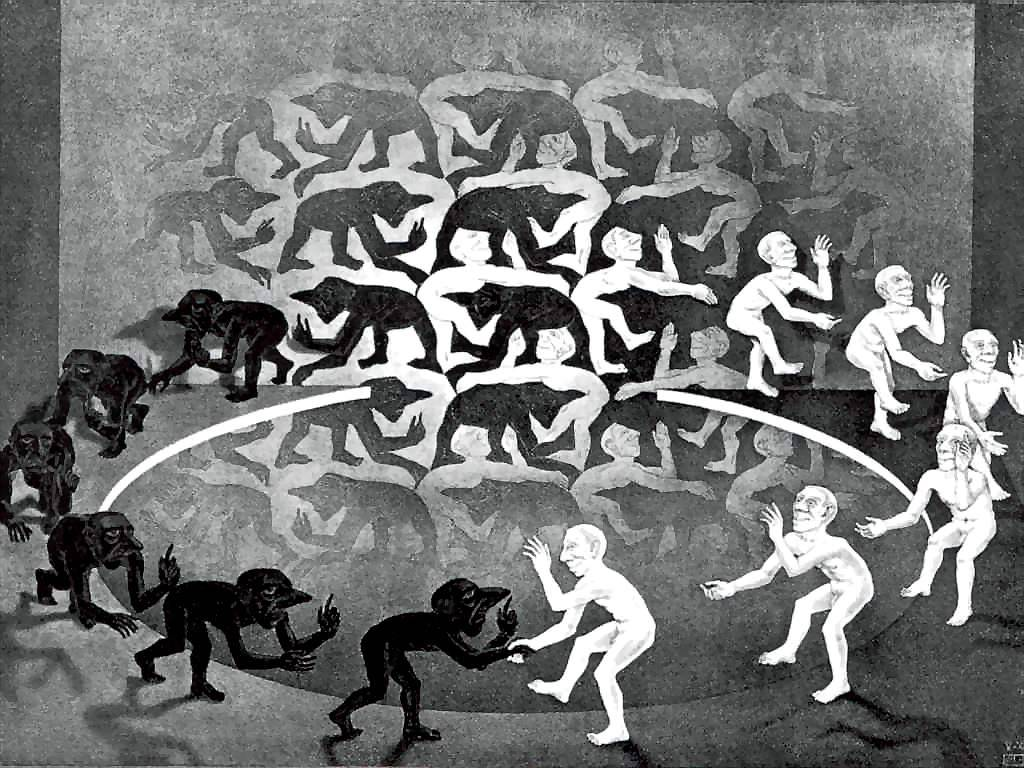
\includegraphics[scale=0.37]{escherEncuentro}

%----------------------------------------------------------------------------------------

\vfill % Fill the rest of the page with whitespace

\end{titlepage}

% ---------------------------------------------------------------------------------------
%         HEADER
%----------------------------------------------------------------------------------------

\fancyhead[L]{Favio Vázquez}
\fancyhead[R]{\thepage}

%----------------------------------------------------------------------------------------
\setcounter{footnote}{0}
\renewcommand*{\thefootnote}{\arabic{footnote}}
%----------------------------------------------------------------------------------------

%----------------------------------------------------------------------------------------
%%			BEGIN DOCUMENT
%----------------------------------------------------------------------------------------

\section{Problema 1}

Explica en que consisten las siguientes técnicas para medir el índice de refracción complejo:

\begin{itemize}
 \item Elipsometría.
 \item Reflectancia, absorbancia y transmitancia.
 \item Técnica de Corbino.
 \item EELS (electron energy loss spectroscopy).
 \item REELS (reflection electron energy loss spectroscopy).
\end{itemize}

\vspace{.3cm}

\underline{Solución:} \vspace{.3cm}

\textbf{Elipsometría}: La elipsometría es una técnica que mide el cambio en los 
estados de polarización de la luz reflejada en la superficie de una muestra. Los 
valores medidos son expresados como $\Psi$ y $\Delta$. Estos valores están relacionados 
con la tasa de los coeficientes de reflexión de Fresnel, $R_P$ y $R_S$ para la 
luz polarizada de tipo $P$ y $S$ respectivamente, y esta relación se expresa 
en la siguiente ecuación 

\begin{equation}
 \tan{\Psi} \euler^{i\Delta} = \frac{R_P}{R_S}.
\end{equation}

Debido a que la elipsometría mide la tasa de los dos valores, puede ser altamente 
precisa y muy reproducible. De la ecuación anterior vemos que la tasa es un 
número complejo, por lo que contiene la información de la fase contenida en $\Delta$, 
que hace que la medición sea muy sensible. 

\vspace{.3cm}

\textbf{Reflectancia, absorbancia y transmitancia}: La reflectancia $\rho$ está definida 
por la tasa de potencia radiante reflejada a la potencia radiante incidente. Para 
un cierto elemento de área $dA$ de la superficie reflectante, la potencia 
radiante incidente diferencial está dada por la irradiancia de la superficie 
$E_e$ multiplicada por la el tamaño del elemento de superficie, entonces 

\begin{equation}
 dF_{e,\text{incidente}} = E_e dA,
\end{equation}

y la potencia radiante reflectada diferencial está dada por la exitancia $M_e$, 
multiplicada por el tamaño del elemento de superficie, 

\begin{equation}
 dF_{e,\text{reflejada}} = M_e dA,
\end{equation}

por lo tanto 

\begin{equation}
 \rho = \frac{dF_{e,\text{reflejada}}}{dF_{e,\text{incidente}}} = 
 \frac{M_e \cancel{dA}}{E_e \cancel{dA}} = \frac{M_3}{E_e}.
\end{equation}

La reflectancia total es luego subdividida en reflectancia regular $\rho_r$ y 
reflectancia difusa $\rho_d$, que están dadas por las tasa de potencia radiante 
reflejada regular y la tasa de potencia radiante reflejada difusa a la potencia 
radiante incidente. De es esta definición debe ser obvio que 

\begin{equation}
 \rho =  \rho_r + \rho_d.
\end{equation}

La transmitancia de un medio está definida por la tasa de potencia radiante transmitida 
por la potencia radiante incidente. La transmitancia es luego subdividida en 
transmitancia regular $\tau_r$ y transmitancia difusa $\tau_d$. que están dadas por 
las tasa de potencia radiante transmitida regular y la tasa de potencia
radiante transmitida difusa a la potencia radiante incidente. De nuevo 

\begin{equation}
 \tau =  \tau_r + \tau_d.
\end{equation}

La absorbancia de un medio es definida por el radio de potencia radiante absorbida 
por la potencia radiante incidente. 

\vspace{.3cm}

Al estar definidas como tasas de los valores de potencia radiante, la reflectancia, 
transmitancia y absorbancia son adimensionales. Estas cantidades son usadas 
para describir propiedades ópticas de los materiales, como el índice de refracción. 
Comúnmente estas cantidades se aplican a radiación compleja, pero también pueden 
utilizarse para radiación monocromática. 

\vspace{.3cm}

\textbf{Técnica de Corbino}: Esta técnica fue desarrollada para proveer la 
respuesta dependiente de las frecuencias  para el rango espectral de microondas. Ha 
sido usada para dar información importante sobre superconductores de alta 
temperatura, fermiones persados, gafas de electrones y películas superconductoras 
delgadas. En esta técnica uno mide los coeficientes de reflexión complejos desde 
una muestra de película fina que termina una línea de transmisión coaxial. 
Típicamente, el contacto eléctrico es hecho presionando un adaptador de microondas 
modificado contra la muestra con almohadillas de oro en forma de dona, que 
empareja las dimensiones radiales de la línea coaxial. 

\vspace{.3cm}

\textbf{EELS (electron energy loss spectroscopy)}: EELS es una técnica analítica que 
mide los cambios en la energía cinética de los electrones luego de que han interactuado 
con un espécimen. Cuando se hace en un microscopio electrónico de transmisión 
moderno, EELS es capaz de dar información estructural y química de un sólido, con 
una resolución espacial a nivel atómico en casos favorables. La resolución energética 
es típicamente 1 eV pero puede acercase a 0.1 eV si se usa un haz de electrones 
monocromático. 

\vspace{.3cm}

Algunos de los electrones se someterán a dispersión inlástica, que significa que 
perderán energía y sus caminos serán pequeñamente deflectados aleatoriamente. La 
cantidad de energía perdida puede ser medida mediante un espectrómetro electrónico 
e interpretada en términos de qué causó la pérdida de energía. Entre estas interacciones 
inelásticas están las ionizaciones de capas internas, que son particularmente 
útiles para detectar los componentes elementales de los materiales. Para estudiar 
superficies, EELS es usualmente usada con bajas energía de incidencia. 

\vspace{.3cm}

\textbf{REELS (reflection electron energy loss spectroscopy)}: REELS es una combinación 
de EELS con microscopía electrónica de reflexión (REM), en la que un haz de electrones 
de alta energía es incidente a un ángulo de brillo sobre la superdicie. Se utiliza 
para estudiar la pérdida de energía de estructuras ``near-edge'' y pérdida de energía 
extendida en estructuras finas de superficies de cristales. También es 
utilizada para detectar cambios relativos en los cambio de estado de densidades 
en superficies.

\section{Problema 2}

Utilizando la transformada de Fourier,encontrar la dependencia en la frecuencia de las siguientes suceptibilidades:

\begin{itemize}
 \item $\chi(t) = \chi_0 \delta(t)$
 \item $\chi(t) = \chi_0\theta(t)$ es la función de Heaviside.
 \item $\chi(t) = \chi_0\delta(t)\sen(\omega_0 t)$.
\end{itemize}

\vspace{.3cm}

\underline{Solución:} \vspace{.3cm}

\section{Problema 3}

Utilizando el modelo de Lorentz para la función dieléctrica muestra que 

$$
\int_0^\infty d\omega \omega \text{Im}(\epsilon(\omega)) = \frac{\omega_p^2}{8}.
$$

En CGS.

\vspace{.3cm}

\underline{Solución:} \vspace{.3cm}

\section{Problema 4}

Plasmones-polaritones de superficie. Supongan que para $z > 0$ hay un metal descrito por el modelo de plasma. Es decir 

$$
\epsilon(\omega) = 1 - \frac{\omega_p^2}{\omega^2}.
$$

Para $z < 0$ hay vacío. Es decir la superficie que divide el metal del vacío es el plano $x - y$.

\begin{itemize}
 \item ¿Qué es un plasmón-polaritón de superficie?
 \item Encontrar la relación de dispersión para el plasmón.
\end{itemize}

\vspace{.3cm}

\underline{Solución:} \vspace{.3cm}

\end{document}